\documentclass[12pt,letterpaper]{article}
\usepackage[margin=1.32in]{geometry} 
\usepackage[utf8]{inputenc}
\usepackage[english]{babel}
\usepackage{amsmath}
\usepackage{amsfonts}
\usepackage{amssymb}
\usepackage{graphicx}
\usepackage{subfigure}
\usepackage{csquotes}
\usepackage{float}
\usepackage{hyperref}

\setcounter{secnumdepth}{5}

\title{Profiling user based on geo-tagged\\socio-temporal data
	\footnote{This project is part of course CS 225: Next Generation Search Systems - Winter 2016, by \href{https://ngs.ics.uci.edu/}{Prof. Ramesh Jain}.}
}

\author{
Karthik Prasad\and Phani Shekhar\and Soumya Mishra
\vspace{2mm}
\footnote{Karthik Rajendra Prasad: Student\# 42686317, Phani Shekhar Mantripragada: Student\# 85686586, Soumya Sucharita Mishra: Student\# 89841518}\\
  University of California Irvine\\
  \texttt{\{prasadkr,pmantrip,ssmishra\}@uci.edu}
}
\date{}


\begin{document}
\maketitle

\begin{abstract}
\noindent
Personalized search results and recommendations rely heavily on the profile of the user. Profile can be defined as a collection of information that captures the person's interests and likes based on his/her activities, behavior, the places frequented, the kind of food consumed and most importantly the profile of the user's friend circle. In this project we propose to build a user's profile by considering user's location information in conjunction with the previous check-ins and users interests. The goal of this project is to be able to associate the user with certain tags by researching on the ways to analyze the geo-tagged socio-temporal data. These tags can then be used by other applications to provide relevant search results and recommendations.
\end{abstract}

\section{Introduction}
The advent of online social-networks and smart-phones have changed the landscape of the way people share information with each other. The widespread presence of these smart-phones with access to the world wide web has essentially created a web of sensors that help create, propagate and process large amounts of data. This hand-held device can not only get information about the user, but also tap into and contribute to a cloud which captures information from multiple such users. By combining what user input and interests with that of the other’s inputs gives valuable insight into the user which can then be used to serve her/him better.
\\\\
One of the primary indicators of user’s personality is the places visited by the person. Many companies such as Foursquare, Facebook, Twitter, Instagram allow geo-tagging to be able to link user’s experience to a point on the map. Not only does this help understand the user’s interests, it also helps annotate the place with the activities performed by the user in that place.

\section{Motivation}
With any system involving user interaction, the scenario is always that of user requiring certain information or service, i.e. having some intention which they want the system to fulfill. Traditional information retrieval systems rely on user being proactive and feeding their inputs mostly in textual/audio form to the system and the system then reacting to this query to generate results. This limits the effectiveness of the search system as -
\begin{enumerate}
  \item User is expected to feed information to the system. This forces the user to come up with a concise query for what they want from the system. As a result, a lot of contextual information about the user which cannot be expressed in the single query but might help serve the user better, is lost.
  \item Most of the current search systems limit the user to express their intent through textual data. However text is not the best way to express the user’s intent as how user’s combine terms to express their query has heavy dependence on linguistics. Thus a user whose native language is french might formulate a search differently from a native english speaker as highlighted in \cite{languagegap}
\end{enumerate}

Thus there is a need to develop search systems that\\
a) are proactive rather than reactive to the user’s intent. Such systems must monitor the user’s surroundings and gain contextual information about the user to better formulate search queries and retrieve accurate results, and\\
b) formulate a new form a query language that is not restricted to user typing words to retrieve results.
\\\\
Work has already been done in coming up with new query languages that bridge the semantic gap between the user and the system through Latent Semantic Analysis \cite{lsa}. Furthermore, with the advent of online social-networks and smart-phones, one can now gain a lot more contextual information about the user such as the location from where the user requested a service, time when information was required, search history etc, that can address the above problem of lack of context in search queries. In addition, hand-held devices can not only get information about the user, but also tap into and contribute to a cloud which captures information from multiple such users. By combining what user input and interests with that of the other’s inputs gives valuable insight into the user which can then be used to serve her/him better.

\section{Novelty of Proposed System}
Our aim is to identify a method that effectively captures the user’s intent to use any system by capturing features that uniquely identify that user and their intent. These features which are represented by tags, will then serve as a new form of querying the system hence provide accurate results. 
We have demonstrated the concept of information retrieval through user-profile tag based querying, in our application Ellipse.
\\\\
Ellipse is a hyperlocal recommendation system that considers the user’s location and experience related to the check-in at that location to generate tags that identify the user’s interest. These tags are then used to recommend events to the user. The central idea of our system is generation of the user profile tags. The profile of the user will not be static information but instead be contextual and vary dynamically based on user’s experience at various locations s/he checks-in to. Furthermore, the profile will be generic that can be used by any recommendation engine irrespective of the domain. We demonstrate the independence of user-profile tags in querying various information systems by using tags created by Ellipse to fetch recommendations for events from the Eventful and Meetup.
\\\\
The highlight of our system is cross-domain utilization of tags. For instance, if a person is involved in health related activities on multiple locations, say Salad bars, beaches or in cafeterias, our system will attempt to tag the user under \enquote{health} so that an event about fitness and health can be suggested by a recommendation system despite the event having nothing to do with food or beaches. The success of this approach is discussed in the Evaluation section of this report.

\section{Technology}
\subsection{Relevant Research Work}
Location based social networks (LBSN) have been extensively studied because they bridge the gap between the social and physical world. Most of the research in this area has been to understand and model three types of graphs : User-user graph, location-location graph and user-location graph. User-user graph tries to model find similar users based on location history, location-location graphs try to model the correlation between locations based on the user’s travel experiences \cite{lbsn}.
\\\\
User’s location history has been used to recommend friends and similar locations \cite{zheng}. \cite{socialties} tries to find user similarity based on semantic meaning of location history and also shows semantic meaning can help identifying overlap between user without overlap in geographic spaces. \cite{travel} uses user’s location history to recommend interesting places and travel sequences using a collaborative filtering technique for unvisited location. There also has been extensive research on point of interest (POI) recommendation on LBSNs by exploring the spatial-temporal patterns. \cite{gao} uses content information and POI properties associated with user check-in to improve recommendation. \cite{geosoca} uses categorical information in addition to the geographical and social correlation between locations for POI recommendations. 
\\\\
Studies have also been conducted in building user profiles based on their interaction with the web \cite{userprofileweb}. Research by Yu, Liu and Zhao represents user’s profile as a collection of concepts and relations between these concepts. The concepts and relations are formulated based on the user’s browsing history. However, this model is restricted to the user’s interaction with the web through feeding search terms into the search engine and misses out on interactions made subconsciously by moving to different locations and use of personal apps available on the cloud. Our approach extends on the work above by considering the use of smartphones to continually sense the user’s environment such as location and use of location discovery and participatory applications to gain contextual information about the user that may further assist in improving search results. 
\\\\
Research has been done in the domain of wireless networks to use the concept of tags to query locations/services of interest and link users with similar tags\cite{patent}. The paper uses tags as keywords to discover services. In our approach, we extend the concept of tag generation to include some level of intelligence, where tags relevant to the user’s interests are created.
\\\\
The concept of using user intent to discover more information has been discussed by Crandall et. al \cite{mapphotos} to identify location of photos clicked by Flickr users. We have adopted a similar approach of using user-intent to find user’s interest. 
\\\\
\cite{clusterfoursquare} discusses using location information to profile users. Thus users who checked into similar places were categorized as having similar interests.

\subsection{Technologies Used}
Since ellipse aims to capture contextual information about the user proactively, without the user having to feed all the information, we decided to build it as a mobile application for Android platform. The app will sense the user’s location through Android’s native geotagging functionality. The user’s experience at the places s/he visits is captured using Krumbs SDK \cite{krumbs}. We propose that a user’s profile is related to the places s/he frequently visits. Thus information about the places where the user checks in should contribute to the user profile tag creation. We obtain this information from Foursquare -- a local search and discovery service. For recommendations on events, we query events discovery services -- Meetup and Eventful. We have used a our custom ranking algorithm to find and order relevant tags of a user.
\\\\
Details of the platforms used are presented below:
\subsubsection{Krumbs SDK}
The Krumbs Software Development Kit (SDK)[7] is a set of tools offered by the Krumbs Platform that enables applications to be built that realize Participatory Sensing.  It is comprised of a set of software modules (client-side and server-side) that enable apps to capture events/moments and all related sensory context (what, where, when , why, who) from a mobile device.  Capture is initiated by the user (mobile device owner)  taking a photo with the device camera (Front or Back) using the K-Capture module. This captured information, represented as \enquote{Krumbs media-JSON},  is auto-uploaded to the Krumbs Cloud Services, where it can be retrieved and used (via the Krumbs API) for search, navigation, query, aggregation and big data analytics. One of the unique features of the client SDK is its ability to capture ‘Intent’ (the 'Why'), with the use of Emojis. These emojis are customizable in the K-Intent Panel SDK component. Applications can define their own Intent Panels that are relevant for their domain. ellipse uses 2 customized intent panels, one for Food and the other for Entertainment. The food panel has 3 emotions associated with it i.e. Yum, neutral and dislike. Entertainment panel has 4 emotions namely - Happy, Love, Neutral and Yawn to indicate degrees of pleasure/displeasure with a particular check-in.

\subsubsection{Mongo DB}
MongoDB is a cross-platform document-oriented database. Classified as a NoSQL database, MongoDB eschews the traditional table-based relational database structure in favor of JSON-like documents with dynamic schemas (MongoDB calls the format BSON), making the integration of data in certain types of applications easier and faster.

\subsubsection{Heroku}
Heroku is a cloud platform as a service. Heroku enables developers to host applications without having to worry about server infrastructure, deployment, ongoing operations, or scaling. 

\subsubsection{Foursquare}
Foursquare is a local search and discovery service mobile app which provides search results for its users. By taking into account the places a user goes, the things they have told the app that they like, and the other users whose advice they trust, Foursquare provides recommendations of the places to go around a user's current location \cite{fsapi}

\subsubsection{Eventful}
Eventful is an online calendar and events discovery service owned by CBS Corporation. The service allows users to search for and track upcoming entertainment events in their area (such as concerts, festivals, and film presentations) involving specific performers, indicate and share their intent to attend certain events, and indicate their "demand" for certain acts to appear in their region. Users can search for events worldwide by time, location, performer, and descriptive keyword. Users can create private or public calendars, including "smart" calendars which automatically update when events matching search criteria are added or existing events are modified.

\subsubsection{Meetup}
Meetup is an online social networking portal that facilitates offline group meetings in various localities around the world. Meetup allows members to find and join groups unified by a common interest, such as politics, books, games, movies, health, pets, careers or hobbies. Users enter their city or their postal code and tag the topic they want to meet about. The website/app helps them locate a group to arrange a place and time to meet. Topic listings are also available for users who only enter a location. \cite{meetupapi}


\section{System Architecture}
\subsection{Application Interaction}
The current idea of the user interaction with the applciation is envisioned as shown in Fig. \ref{fig:appinter}.
\\\\
The user opens the app and checks in to a place. Further, the user input's his/her intent and activity at that place. The application gathers extra information about the location by issuing an API call to foursquare and maintains a user profile. When the user opens the app at a later time and seeks recommendations, the application pings the backend server which issues API requests to eventful and meetup to obtain a list of events most relevant to the user based on the user profile.
\begin{figure}[H]
	\centering
	 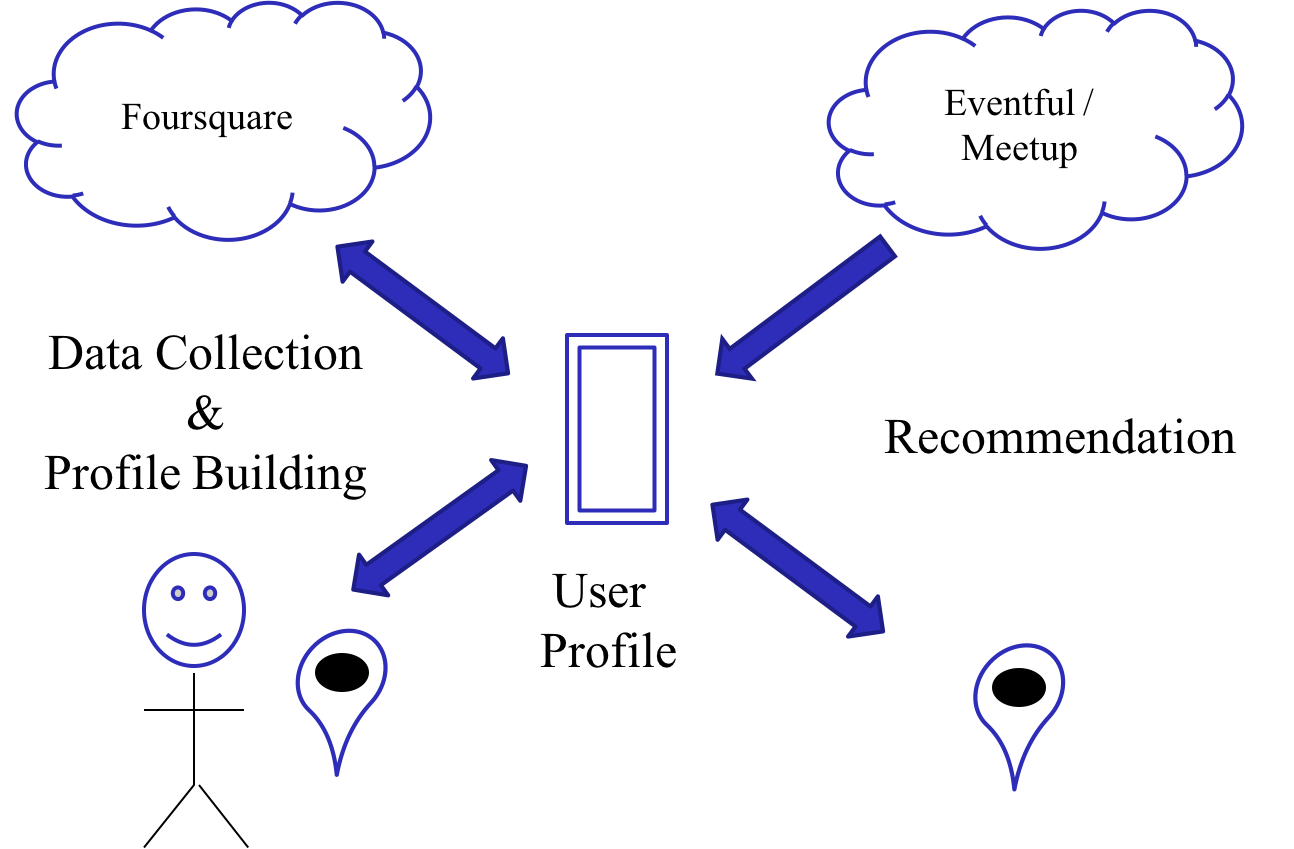
\includegraphics[width=\textwidth, height=9cm]{img/appinter.png}
	 \caption{Application Interaction}
  	 \label{fig:appinter}
\end{figure}

\subsection{System Components}
The interactions of different components of the system are shown below (Fig. \ref{fig:syscomp}) .
\begin{figure}[H]
	\centering
	 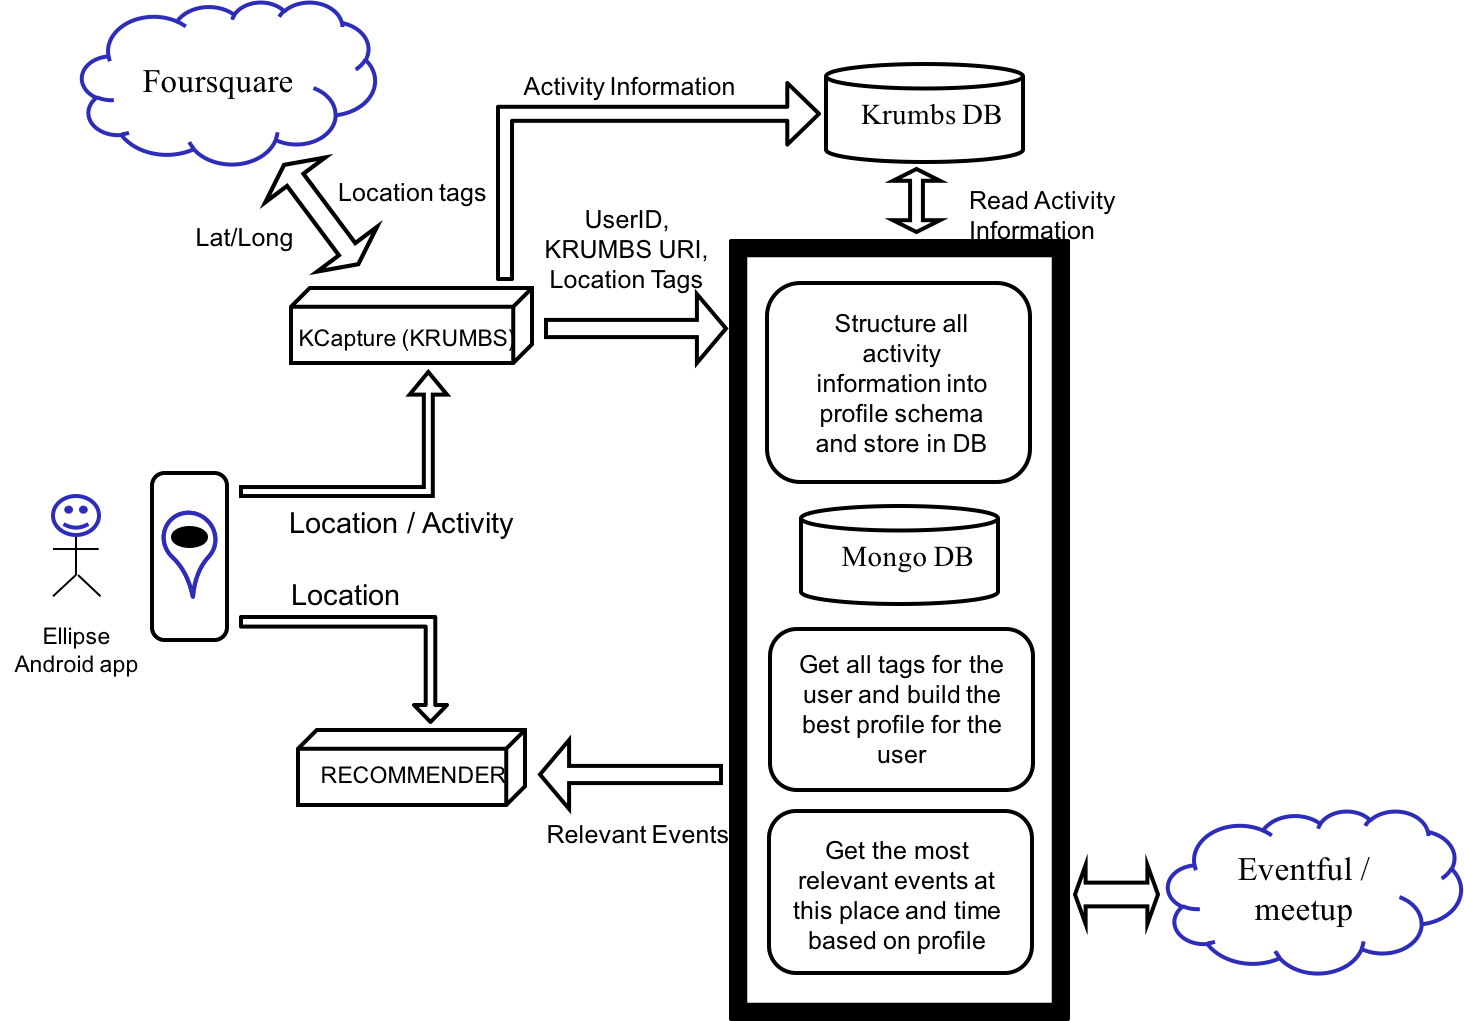
\includegraphics[width=\textwidth, height=9cm]{img/syscomp.png}
	 \caption{System Components}
 	 \label{fig:syscomp}
\end{figure}
\begin{enumerate}

\item \textbf{Front End (User’s Device)}
	\begin{itemize}
	\item Krumbs SDK Capture -- captures the user's activity along with the reaction. It also fetches the location related tags for from Foursquare and POSTs the data to the backend server
	\item Recommendation -- sends the user ID and the current location to the back-end server and GETs the event recommendation from the server.
	\end{itemize}
\item \textbf{Back End Server}
	\begin{itemize}
	\item Check-in Handler -- handles the POST data from the client.
	\item MongoDB database -- stores the user profile information based on check-ins.
	\item Tag Scoring Algorithm -- build a user profile by aggregating and processing user check-in information and generates a set of representative tags.
	\item Recommendation Request Handler -- fetches the most relevant events for the user based on the user profile from eventful and Meetup and pushes the data to the client. 
	\end{itemize}
\end{enumerate}

\section{System Implementation}
As seen in System Architecture \ref{fig:syscomp}, the system can be broadly divided into Client Mobile Application and Backend Server.

\subsection{Client Mobile Application}
We built a mobile application for Android OS \cite{android} that consists of two main components : Capture component and Recommendation. They can be accessed from the homescreen as shown in Fig. \ref{fig:home}

\subsubsection{Capture}
The capture component captures relevant information about user’s check-in and sends the obtained information in a Json format mentioned below to the backend server through http POST.
{ \enquote{uid}: user\_id, \enquote{krumbs}: Krumbs\_URI, \enquote{loc\_tags}: [loc\_tag1, loc\_tag2, ...] }
\\\\
The User ID is the user’s gmail ID registered with the Android device obtained using Android AccountManager API. The rest of the information is obtained from the following two components.

\paragraph{K Capture}\mbox{}\\
Capture component captures information about user’s activity during a check-in using Krumbs SDK. Krumbs SDK provides K-Capture component for capturing moments in terms of user’s location, intent, audio, image and caption.  K-Intent panel is customized for the purpose of our application as shown in Fig. \ref{fig:kcapture}. User’s check-in can fall into the intent categories of Food, Entertainment and Sports. In each of the intent categories, there are intents which the user would select to express the specific intent. For example, the \enquote{Food} intent category has intents like \enquote{Yum}, \enquote{Neutral} and \enquote{Dislike}. These intents are specifically designed to capture the mood of the user during the check-in.
\\\\
After user captures an image from the screen containing K-Intent panel, audio can be optionally captured and edited. A auto-generated caption is generated which the user can edit. For the purposes of our application, we expect the user to input tags related to the user’s activity as part of the caption. This will result in the complete capture of user’s intent as part of the check-in.  This check-in data can be accessed from a unique URL in the format of Json data. This URL forms the \enquote{krumbs} part of the request to the back-end server.

\paragraph{Foursquare API}\mbox{}\\
The second part of the Capture component tries to collect information about the check-in location. For this purpose, FourSquare API is used. Foursquare is a local search and discovery service mobile app which provides search results for its users. Foursquare search API endpoint, \enquote{https://api.foursquare.com/v2/venues/search} gives a list of possible venues and their meta-data based on geo-location. From this list, the user’s venue is picked using the intent from K-Capture component. The metadata contains the category of the venue. For example, the category associated with \enquote{StarBucks} would be \enquote{Coffee Shop}. This category information forms the \enquote{loc\_tags} part of the request to the back-end server.

\subsubsection{Recommendation}
The recommendation component is activated when user clicks on the recommend button in the home screen. It fetches event recommendations from the back-end server through a GET request. As part of the request, the user ID, obtained from the device and geolocation is sent as parameters. These results are displayed to the user using android cards as shown in Fig. \ref{fig:uireco}. Each card displays the title and description about the event and optionally if it is a trending event. On clicking the card, the user is redirected to the event Web Page containing additional details like time,venue etc.

 \begin{figure}[H]
	      	\centering
	      	\subfigure[Homescreen]{
	      		
\includegraphics[width=0.30\textwidth, height=3.3in]{img/home.jpg}
	      		\label{fig:home}		            
	      	}				
	      	\subfigure[KCapture]{
	      		
\includegraphics[width=0.30\textwidth, height=3.3in]{img/food.jpg}
	      		\label{fig:kcapture}
	      	}
	      	\subfigure[Recommendation Page]{
	      		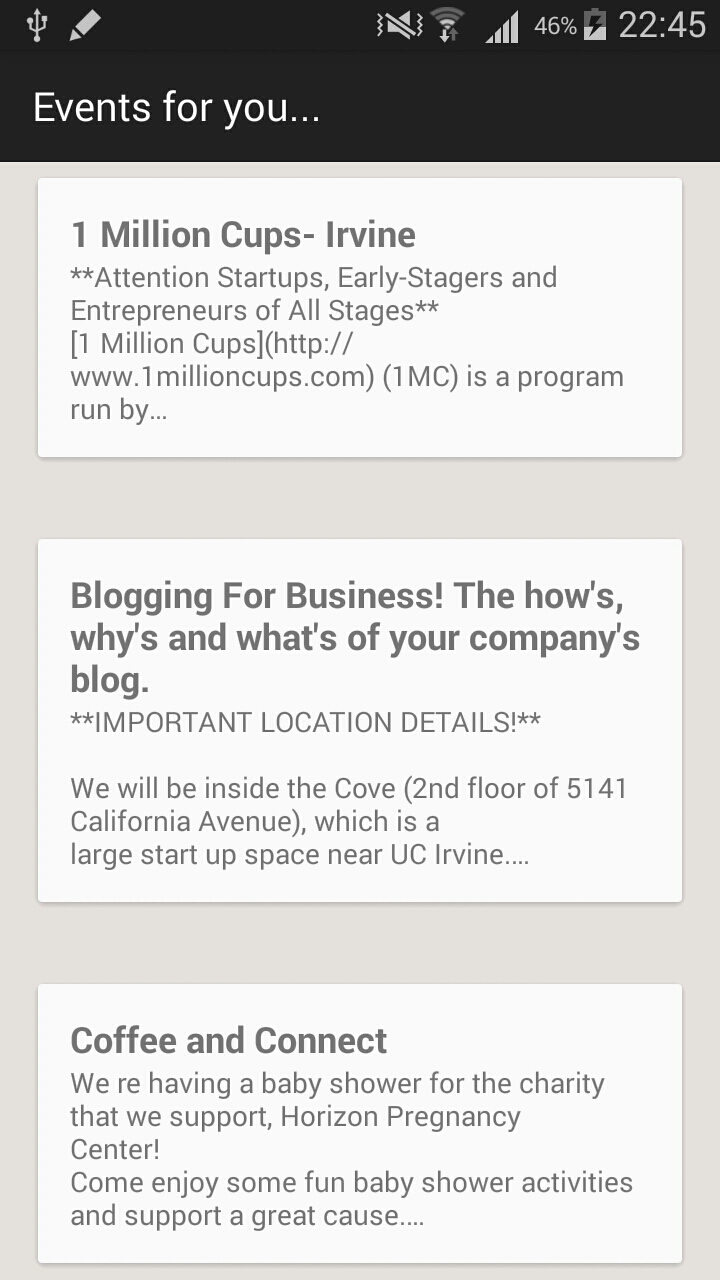
\includegraphics[width=0.30\textwidth, height=3.3in]{img/uireco.jpg}
	      		\label{fig:uireco}
	      	}
	      	\caption{Ellipse Application UI}
	      	\label{fig:ui}        			
\end{figure}

\subsection{Back-End Server}
The system uses a backend server developed in Python's Flask framework \cite{flask} and acts as a single point of contact for the mobile app running on different devices. The web server handles storage of user activity information in a centralized data base and also runs the algorithm to build a user profile. Further, a back-end server process fetches the relevant event recommendations (based on user profile) and ranks them before pushing to the device.
\\\\
The initial implementation approach aimed to decentralize the above process by keeping the implementation of the business logic and user data base with the client. We rejected this as it made the client logic heavy and inflexible. Further, pushing the logic to a centralized server allows scalability on a distributed setup and open frequent updates. Additionally, a centralized database of all user data can help identify identical user profiles and check-ins to further improve personal profile and personalized recommendations.
\\\\
The individual components are discussed in detail below:
\subsubsection{Check-in Handler}
The check-in handler accepts an http POST body with user\_id, Krumbs URI and location\_tags for a particular check-in. The server then contacts Krumbs database using the Krumbs URI and gathers activity information for that check-in. The relevenat information such as Who (user\_id), Where (location lat/long), When (timestamps), Which (category name and reaction), What (activity as input by the user) along with tags describing the location (fetched from foursqaure) are extracted, massaged and stored in to the database.

\subsubsection{User Profile Database}
We are using a MongoDB -- a No-SQL database -- to store the information gathered from the user's devices. This was an obvious choice given the nature of data that is being stored. No-SQL database does not force us to stick to a schema which can change frequently over the course of development of this system. MongoDB is an opensource No-SQL database with high-perfromance, easy scalability and an expressive query language (CITE https://www.mongodb.com/scale/database-software-open-source). 

Each document (i.e., row) in the database has the following format:\\
\\
\{\enquote{uid}:user\_id, \enquote{tag}:tag, \enquote{check-in\_info}:[\(check-in_1, check-in_2, ..., check-in_n\)]\}\\
\\
\(check-in_i\) = \{\enquote{timestamp}: timestamp, \enquote{loc}: lat,long, \enquote{category}:category, \enquote{emotion}:emotion\_score, \enquote{tag\_type}:\enquote{a}$|$\enquote{l}\}
\\\\
Each <user,tag> pair has one row in the database and captures a list of information of the user's check-in associated with the tag, i.e., in effect, <user\_id, tag> pair is a primary key of this database. Each check-in information captures the time when the check-in occurred, the location of the check-in, the category of the activity performed by the user during that check-in as well as the user's emotional reaction to the activity. We also store the information about whether that tag is associated with the user's activity (type "a") or the location (type "l").
\\\\
The emotional reaction is a score on the scale of -5 to +5 assigned to each emoji in the KCapture component. For example, in category \enquote{Food}, we have three emotions: \{\enquote{Yum}, \enquote{Neutral}, \enquote{Dislike}\} with corresponding emotion scores as \{-1,1,2\}. Similarly, we have emotion scores for every reaction in every category. The mapping of emotion to scores are controlled on the back-end and can be tweaked to build accurate profiles.

\subsubsection{Tag Scoring Algorithm}
The tags gathered from the user's check-ins -- both activity as well as the location -- represent the user's interests and hence can be constituents of a user profile. However, the task of assigning relevance scores to each of them is non-trivial.  Not every activity is a sign of user interest. Some of the check-ins might just be a one time activity and not really a representative of user's interest. However, they still carry some weight as it could be the case that the user is exploring new interests. 
\\\\
Similarly, an activity which has got a negative reaction from the user is not a valid constituent of user profile. Furthermore, non occurrence of an activity for a long time could be an indicator of dying significance of that constituent. In other words, the constituent of a user profile has a life time and needs to be reinforced to be relevant to the user. For instance, if a user who frequented bars turned non-alcoholic and stops check-ins form the bars, it indicates that his/her interest in alcohol has decreased and hence are not indicative of the user anymore. 
\\\\
Additionally, the life time of a tag depends on the category of activity associated with the tag. Sporting events happen less frequently than movie releases. Therefore, non occurrence of a sports related tag for a long time cannot be construed as non-relevant even though its true for movies.
\\\\
In summary, the following factors affect the relevance score associated with a tag: time of trigger, the number of triggers, the emotion associated with each trigger and the category of the tag among others. The two main components of scoring, therefore, are the frequency component and time-related decay component. Our scoring formula for a tag is

\[\frac{I_0}{n} \left( w_f f_t + w_d d_t \right) \]
where,\\
\(I_0\) is the initial score of the tag \(t\),\\
\(n\) is the number of check-ins associated with the tag \(t\),\\
\(w_t\) is the weight of the tag frequency score,\\
\(f_t\) is the frequency of tag \(t\),\\
\(w_d\) is the weight of the time-decay score,\\
\(d_t\) is the time-decay score of the tag \(t\).
\\\\
The power law distribution accurately describes the decay score of the tag and captures all of the above factors correctly. The decay score is given by 
\[d_t = \sum_{c} r_c e^{-\lambda _k \Delta t} \]
where,\\
\(d_t\) is the score associated with a time-decay for tag \(t\),\\
\(r_c\) is the reaction/emotion associated with the check-in \(c\),\\
\(\lambda_k\) is the decay rate for category \(k\),\\
\(\Delta t\) is the time elapsed between the occurrence of the check-in and now.
\\\\
The above algorithm gives a score for each tag of the user; higher the score, higher the relevance to the user at a given point in time.

\subsubsection{Recommendation Request Handler}
The back-end server exposes an HTTP GET request handler to deliver recommendations. It accepts the user ID and the user's current location as an input. It then obtains the most relevant tags for the user in the order of relevance from the User profile database. A list of recommended events are obtained from both Eventful and Meetup using these most relevant tags. Along with the events obtained using user tags, a list of trending events in the locality are also fetched as they might interest the user even if they do not match user profile. This is to facilitate the user to explore new interests . All these results are aggregated into JSON format and sent back to the client android application. 

\section{System Evaluation}
\subsection{Performance Improvements}
\begin{enumerate}
\item Initially, all the components are thought be a part of the android application. In order to optimize on the computational resources used by the app and to facilitate offline pruning of user tags, some components have been moved to a back end server. 
\item The schema of the database has been changed from a initial design of a new row per check-in to a row per tag per user containing list of check-in meta-data. This helped in faster processing of recommend requests. 
\item Eventful and MeetUp APIs are queried using a set of tags even though the API does not honor prominence among them. An alternative to this would be query the endpoints individually for each tag. But this approach was expensive as each query to the endpoint would take about 0.2 sec approximately. So, after the results are obtained for a bag of tags, they are ordered using ranking of tags occurring in their descriptions.
\end{enumerate}

\subsection{Recommendation Improvements}
The relevant tags of the user are extended to fetch better event recommendations using \emph{synsets} and \emph{hypernyms} from WordNet \cite{wordnet}. For each tag, a set of synonyms can be obtained using \emph{synsets}. For each item in this list, the \emph{hypernyms} and their \emph{lemma} names gives a hierarchy of these tags. These tags extend the possible activities of interest of the user. For example, user tags of Cappuccino and Latte are extended with the tag Coffee to improve the suggestions.

\subsection{Results}
Given below is a list of use cases of user check-in and the prominent tags estimated by the system.
\begin{enumerate}
\item User check-in contains salad bar, subway, swimming etc. with captions such as healthy living etc. in most of them. The system assigns the tag \enquote{health} as the most important one and fetches recommendations related to health.
\item User check-in contains unrelated captions like reading, chilling, meeting with friends etc. at multiple pizza places. The system assigns a higher rank to "pizza" than the activity tags and fetches recommendations happening in pizzeria.
\item If user check-in ranks \enquote{cappuccino} as a high ranked tag, there were no possible recommendations. However, after adding logic to include WordNet, \enquote{coffee} is added to list of tags and multiple coffee related events were listed.
\end{enumerate}

\section{Future Work}
Extending the idea of recommendations based on user’s profile tags, the system should be able to assess tags of the user’s friends who are also in the system and generate recommendations based on common interests between the user and his/her friends. Likewise, one can group users with similar tags (need not be in friend list) and generate recommendations to this group as a whole based on tags of users within each group. Furthermore, tags of users who visit places similar to the places visited by the user can help identifying common interests. However, this is a non trivial problem and is not merely based on simple intersection between different user’s tag set. Future versions of Ellipse aims to improve on these fronts.

\section{Conclusion}
As several advancements are being made in enhancing user’s experience in his/her interaction with software systems, the key to the ultimate user focused application will rely heavily on retrieving as much relevant information about the user as possible. This is where next generation search systems come in play by building on this contextual information and generating new information. We find that user specific contextual information need not be extracted in a standalone fashion native to the search system but can also be extracted from the user’s direct or indirect interaction with other applications. While applications like BookMyShow\cite{bookmyshow} and Zomato\cite{zomato} have done a great job tying up with several vendors and hyper-local services in aggregating all the information the user may need hence making it a one stop user application, such services seem scattered in the location discovery services domain. Our app bridges that gap by connecting the user’s contextual information over several location based services through user-profile tags. These tags provide information about the user’s interest and serve as a new recommendation specific way of querying various data sources.

\begin{thebibliography}{9}

\bibitem{languagegap}
	\enquote{The Wikipedia Language Gap: Understanding and Designing for Global Communities - Darren Gergle. YouTube. N.p., n.d. Web. 16 Mar. 2016.}\textit{Web}.	\href{https://youtu.be/6egCxY-X7Xs?list=PLcm9UtazJCOKbKQugcvWaoz3bLjj925ry}
	{\url{https://youtu.be/6egCxY-X7Xs?list=PLcm9UtazJCOKbKQugcvWaoz3bLjj925ry}}
	
	\bibitem{lsa}
	\enquote{Handbook of Latent Semantic Analysis.} (2014): n. pag. Web.
	
	\bibitem{userprofileweb}	
	2012 International Conference On Innovation And Information Management (Iciim 2012). \textit{Building User Profile Based on Concept and Relation for Web Personalized Services} (n.d.): n. pag. Web.
	
	\bibitem{patent}
	\enquote{Patent Application - Tags for Location-based Services in Wireless Networks Summary.} 	  \textit{Tags for Location-based Services in Wireless Networks.} N.p., n.d. Web. 16 Mar. 2016. \href{https://www.patexia.com/us-publications/20040235493}{\url{https://www.patexia.com/us-publications/20040235493}}
	
	\bibitem{mapphotos}
	\enquote{Mapping the World's Photos.} \textit{Mapping the World's Photos.} N.p., n.d. Web. 16 Mar. 2016. \href{http://dl.acm.org/citation.cfm?id=1526812}{\url{http://dl.acm.org/citation.cfm?id=1526812}}
	
	\bibitem{clusterfoursquare}
	\enquote{Beyond "local", "categories" and "friends": Clustering Foursquare Users with Latent "topics"} \textit{Beyond "local", "categories" and "friends"} N.p., n.d. Web. 16 Mar. 2016. \href{http://dl.acm.org/citation.cfm?id=2370422}{\url{http://dl.acm.org/citation.cfm?id=2370422}}
	
	\bibitem{krumbs}
	\enquote{Krumbs Platform SDK 1.0.0 Documentation.} \textit{Google Docs.} N.p., n.d. Web. 16 Mar. 2016. \href{https://docs.google.com/document/d/1OKxgwaz4_8iHuTi4e0pBtgy1rqfXTdmW9o66JZwhn3c/edit}{\url{https://docs.google.com/document/d/1OKxgwaz4_8iHuTi4e0pBtgy1rqfXTdmW9o66JZwhn3c/edit}}
	
	\bibitem{fsapi}
	\enquote{Introduction to the Foursquare API. N.p., n.d. Web. 04 Feb. 2016.} \textit{Web}. \href{http://www.ibm.com/developerworks/library/os-foursquare/}{\url{http://www.ibm.com/developerworks/library/os-foursquare/}}

	\bibitem{eventfulapi}
	\enquote{Eventful API. N.p., n.d. Web. 04 Feb. 2016.} \textit{Web}. \href{https://api.eventful.com/}{\url{https://api.eventful.com/}}
	
	\bibitem{meetupapi}
	\enquote{MeetUp API. N.p., n.d. Web. 04 Feb. 2016.} \textit{Web}. \href{http://www.meetup.com/meetup_api/}{\url{http://www.meetup.com/meetup_api/}}	

	\bibitem{lbsn}
	\enquote{Location-Based Social Networks. N.p., n.d. Web. 04 Feb. 2016.} \textit{News}. \href{http://research.microsoft.com/en-us/projects/lbsn/}{\url{http://research.microsoft.com/en-us/projects/lbsn/}}
	
	\bibitem{zheng}
	Zheng, Yu, Lizhu Zhang, Zhengxin Ma, Xing Xie, and Wei-Ying Ma. \enquote{Recommending friends and locations based on individual location history.} \textit{ACM. Transactions on the Web (TWEB) 5, no. 1 (2011)}

	\bibitem{socialties}
	Xiao, Xiangye, Yu Zheng, Qiong Luo, and Xing Xie. \enquote{Inferring social ties between users with human location history.} \textit{Journal of Ambient Intelligence and Humanized Computing 5, no. 1 (2014): 3-19.}
	
	\bibitem{travel}
	Zheng, Yu, and Xing Xie. \enquote{Learning travel recommendations from user-generated GPS traces.} \textit{ACM Transactions on Intelligent Systems and Technology (TIST) 2, no. 1 (2011): 2.}

	\bibitem{gao}
	Gao, Huiji, Jiliang Tang, Xia Hu, and Huan Liu. \enquote{Content-Aware Point of Interest Recommendation on Location-Based Social Networks.} \textit{In AAAI, pp. 1721-1727. 2015.}

	\bibitem{geosoca}
	Zhang, Jia-Dong, and Chi-Yin Chow. \enquote{GeoSoCa: Exploiting geographical, social and categorical correlations for point-of-interest recommendations.} \textit{InProceedings of the 38th International ACM SIGIR Conference on Research and Development in Information Retrieval, pp. 443-452. ACM, 2015.}

	\bibitem{android}
	\enquote{Android.} \textit{Android.}	N.p., n.d. Web. 16 Mar. 2016. \href{https://www.android.com/}{\url{https://www.android.com/}}
	
	\bibitem{flask}
	\enquote{Flask.} \textit{Flask.}	N.p., n.d. Web. 16 Mar. 2016. \href{http://flask.pocoo.org/}{\url{http://flask.pocoo.org/}}
	
	\bibitem{wordnet}
	\enquote{WordNet.} \textit{About} - . N.p., n.d. Web. 16 Mar. 2016. \href{https://wordnet.princeton.edu/}{\url{https://wordnet.princeton.edu/}}


	\bibitem{bookmyshow}
	\enquote{BookMyShow. N.p., n.d. Web. 04 Feb. 2016.} \textit{Web}. \href{https://www.bookmyshow.com/}{\url{https://www.bookmyshow.com/}}
	
	\bibitem{zomato}
	\enquote{Zomato. N.p., n.d. Web. 04 Feb. 2016.} \textit{Web}. \href{https://www.zomato.com/}{\url{https://www.zomato.com/}}

\end{thebibliography}




\end{document}
